\chapter{Dermatology}

\section{Introduction}
Skin cancer - the most common human malignancy \cite{society2016cancer, rogers2015incidence, stern2010prevalence} - is primarily diagnosed visually, beginning with an initial clinical screening, followed potentially by dermoscopic analysis, a biopsy, and histopathological examination. Automated classification of skin lesions using images is a challenging task due to the fine-grained variability of skin lesion appearance. Deep convolutional neural networks (CNN) \cite{lecun2015deep, lecun1998handbook} show great promise for general and highly variable tasks over many fine-grained object categories \cite{russakovsky2015imagenet, krizhevsky2012imagenet, ioffe2015batch,  szegedy2016rethinking, szegedy2015going, he2016deep}. I present classification of skin lesions using a single CNN, trained end-to-end directly from images using only their pixels and disease labels as inputs. A CNN was trained on a dataset of 129,450 clinical images - two orders of magnitude larger than previous datasets \cite{masood2013computer} - consisting of 2,032 different diseases. Its performance is tested against 21 board-certified dermatologists on biopsy-proven clinical images with two critical use cases: binary classification of (1) malignant carcinomas versus benign seborrheic keratoses, and (2) malignant melanomas versus benign nevi. Case (1) represents the identification of the most common cancer, and case (2) represents identification of the deadliest skin cancer. The CNN achieves performance on par with all tested experts across both tasks, demonstrating, for the first time, an artificial intelligence with dermatologist-level skin cancer classification capability. Outfitted with deep neural networks, mobile devices can extend the reach of dermatologists outside of the clinic, and enable low-cost universal access to vital diagnostic care. 

There are 5.4 million new cases of skin cancer each year in the United States \cite{rogers2015incidence}. One in five Americans will be diagnosed with a cutaneous malignancy in their lifetimes. While melanomas represent fewer than 5\% of all skin cancers in the United States, they account for approximately 75\% of all skin cancer-related deaths, and are responsible for over 10,000 deaths annually in the United States alone. Early detection is critical - the 5-year survival rate of melanoma drops from 97\% if detected in its earliest stages to 14\% if detected in its latest stages. The key contribution of this work is a computational method which could allow medical practitioners and patients to proactively track skin lesion health and detect cancer early. By creating a novel disease taxonomy and partitioning algorithm which map individual diseases into training classes, a deep learning system is built for automated dermatology. 

Prior work in dermatological computer-aided classification \cite{masood2013computer, rosado2003accuracy, burroni2004melanoma} has lacked the generalization capability of medical practitioners due to insufficient data and a focus on standardized tasks such as dermoscopy \cite{kittler2002diagnostic, codella2015deep, codella2018skin} and histology image classification \cite{binder1998epiluminescence, altmeyer1997skin, clark1989model, schindewolf1993classification}. Dermoscopy images are acquired via a specialized instrument and histology images are acquired via invasive biopsy and microscopy; both of these modalities yield highly standardized images. Photographic images (e.g. smartphone images) exhibit variability in zoom, angle, lighting, etc, making classification significantly more challenging \cite{ramlakhan2011mobile, ballerini2013color}. This challenge is overcome using a data-driven approach - 1.41 million pre-training and training images make it robust to photographic variability. Many former techniques require extensive preprocessing, lesion segmentation, and extraction of domain-specific visual features prior to classification. In contrast, this system requires no hand-crafted features - it is trained end-to-end directly from image labels and raw pixels, with a single network for both photographic and dermoscopic images. The existing body of work uses small datasets of typically less than a thousand skin lesion images \cite{kittler2002diagnostic, codella2018skin, binder1998epiluminescence} that, as a result, do not generalize well to new images. Generalizable classification is demonstrated with a new dermatologist-labeled dataset of 129,450 clinical images including 3,374 dermoscopy images.

Deep learning algorithms, powered by advances in computation and extremely large datasets \cite{deng2009imagenet}, have recently been shown to exceed human performance at visual AI tasks such as Atari game playing \cite{mnih2015human}, strategic board games like Go \cite{silver2016mastering}, and object recognition \cite{russakovsky2015imagenet}. The development of a deep convolutional neural network is outlined that matches the performance of dermatologists at three key diagnostic tasks: melanoma classification, melanoma classification using dermoscopy, and carcinoma classification.  Comparison is restricted to image-based classification.

\section{Methods}

A GoogleNet Inception-v3 CNN architecture \cite{szegedy2016rethinking} is pretrained on ~1.28 million images (1,000 object categories) from the 2014 ImageNet Large Scale Visual Recognition Challenge \cite{russakovsky2015imagenet}, and train it on the collected dermatology dataset using transfer learning \cite{pan2009survey}. Figure \ref{fig:derm_cnn} demonstrates the working system. The CNN is trained on general lesion classification using 757 disease classes. The created dataset is composed of dermatologist-labeled images organized in a novel tree-structured taxonomy of 2,032 diseases, where the individual diseases form the leaf nodes. The images come from 18 different clinician-curated, open-access online repositories as well as clinical data from the Stanford Hospital. Figure \ref{fig:derm_taxonomy}(a) shows a subset of the full taxonomy, which has been organized clinically and visually by medical experts. The dataset is split into 127,463 training/validation images, and 1,942 biopsy-labeled test images.

\begin{figure}
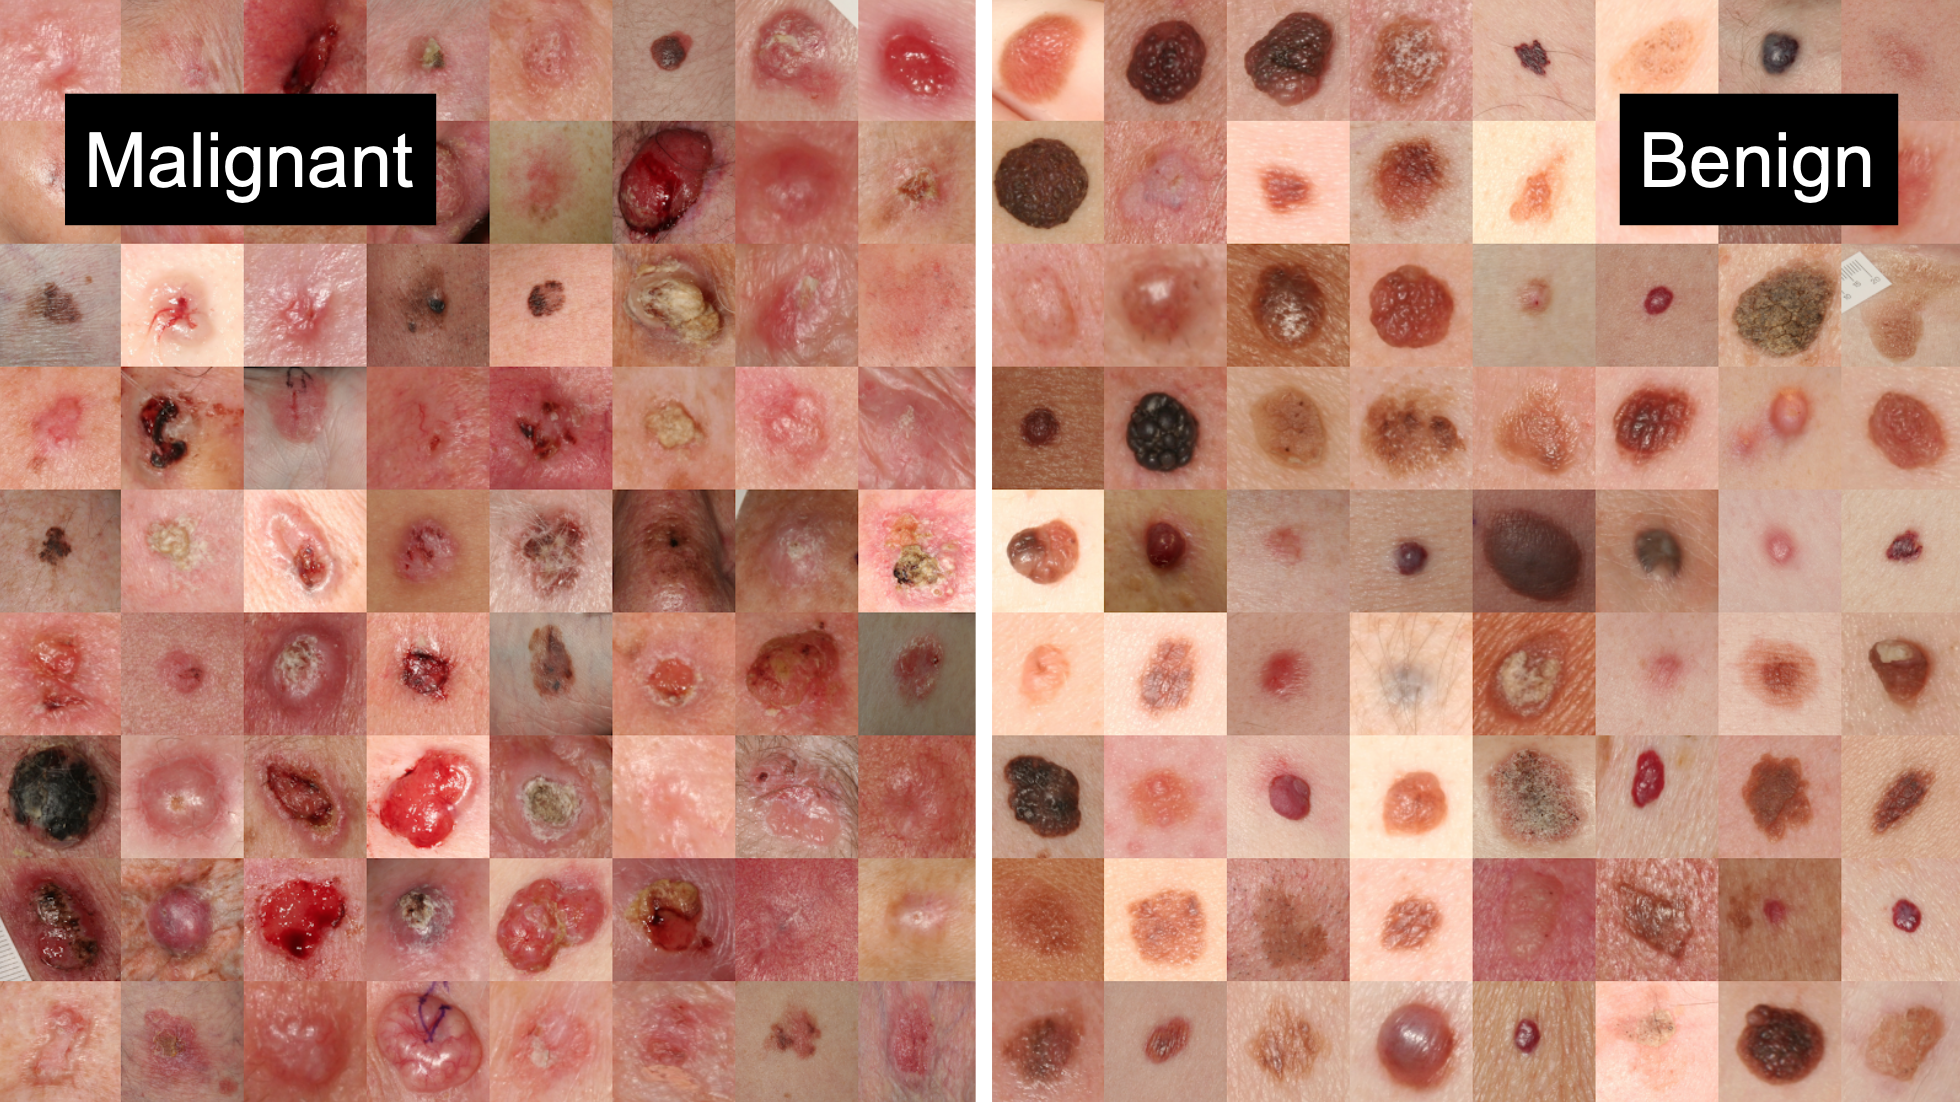
\includegraphics[width=\textwidth]{derm_benign_malignant}
\caption{Benign vs Malignant}
\vspace{12px}
Insert caption here
\label{fig:derm_benign_malignant}
\end{figure}

\begin{figure}
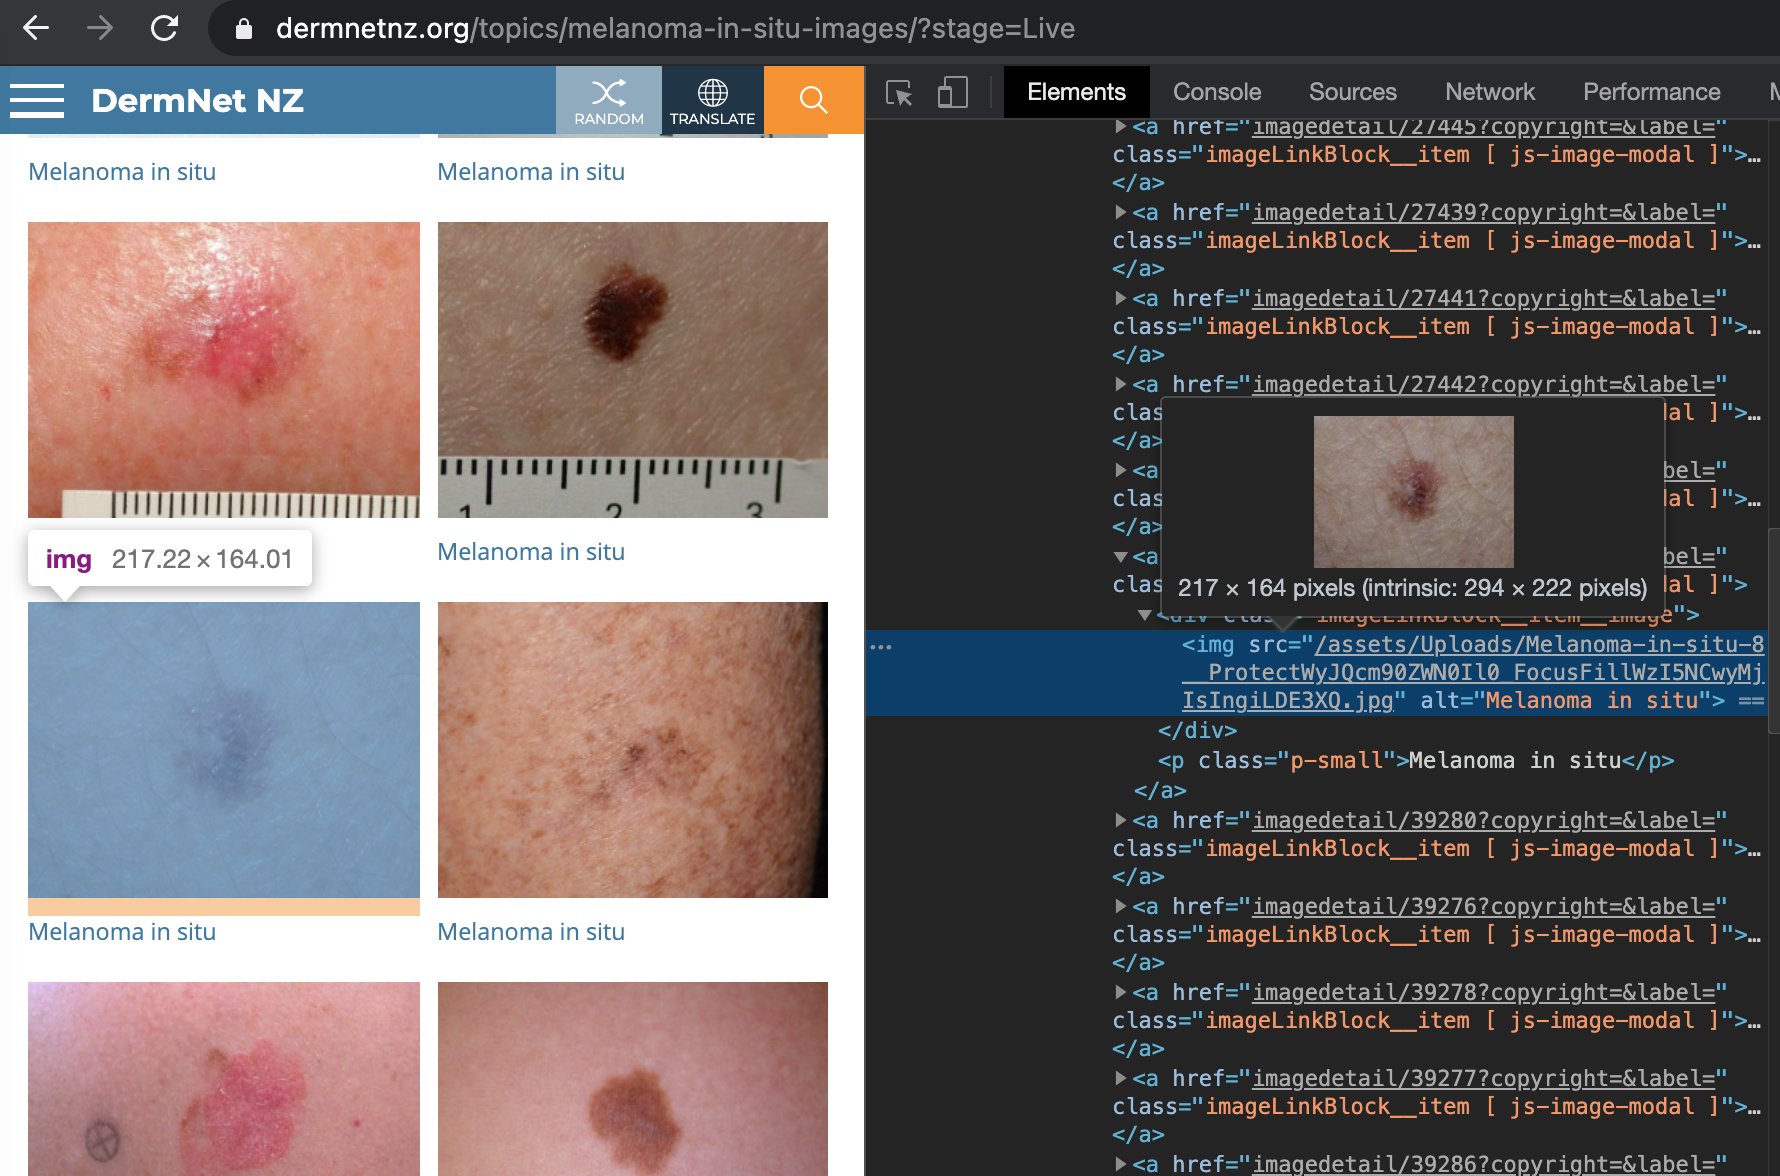
\includegraphics[width=\textwidth]{derm_scrape}
\caption{Data Collection}
\vspace{12px}
Insert caption here
\label{fig:derm_scrape}
\end{figure}

\begin{figure}
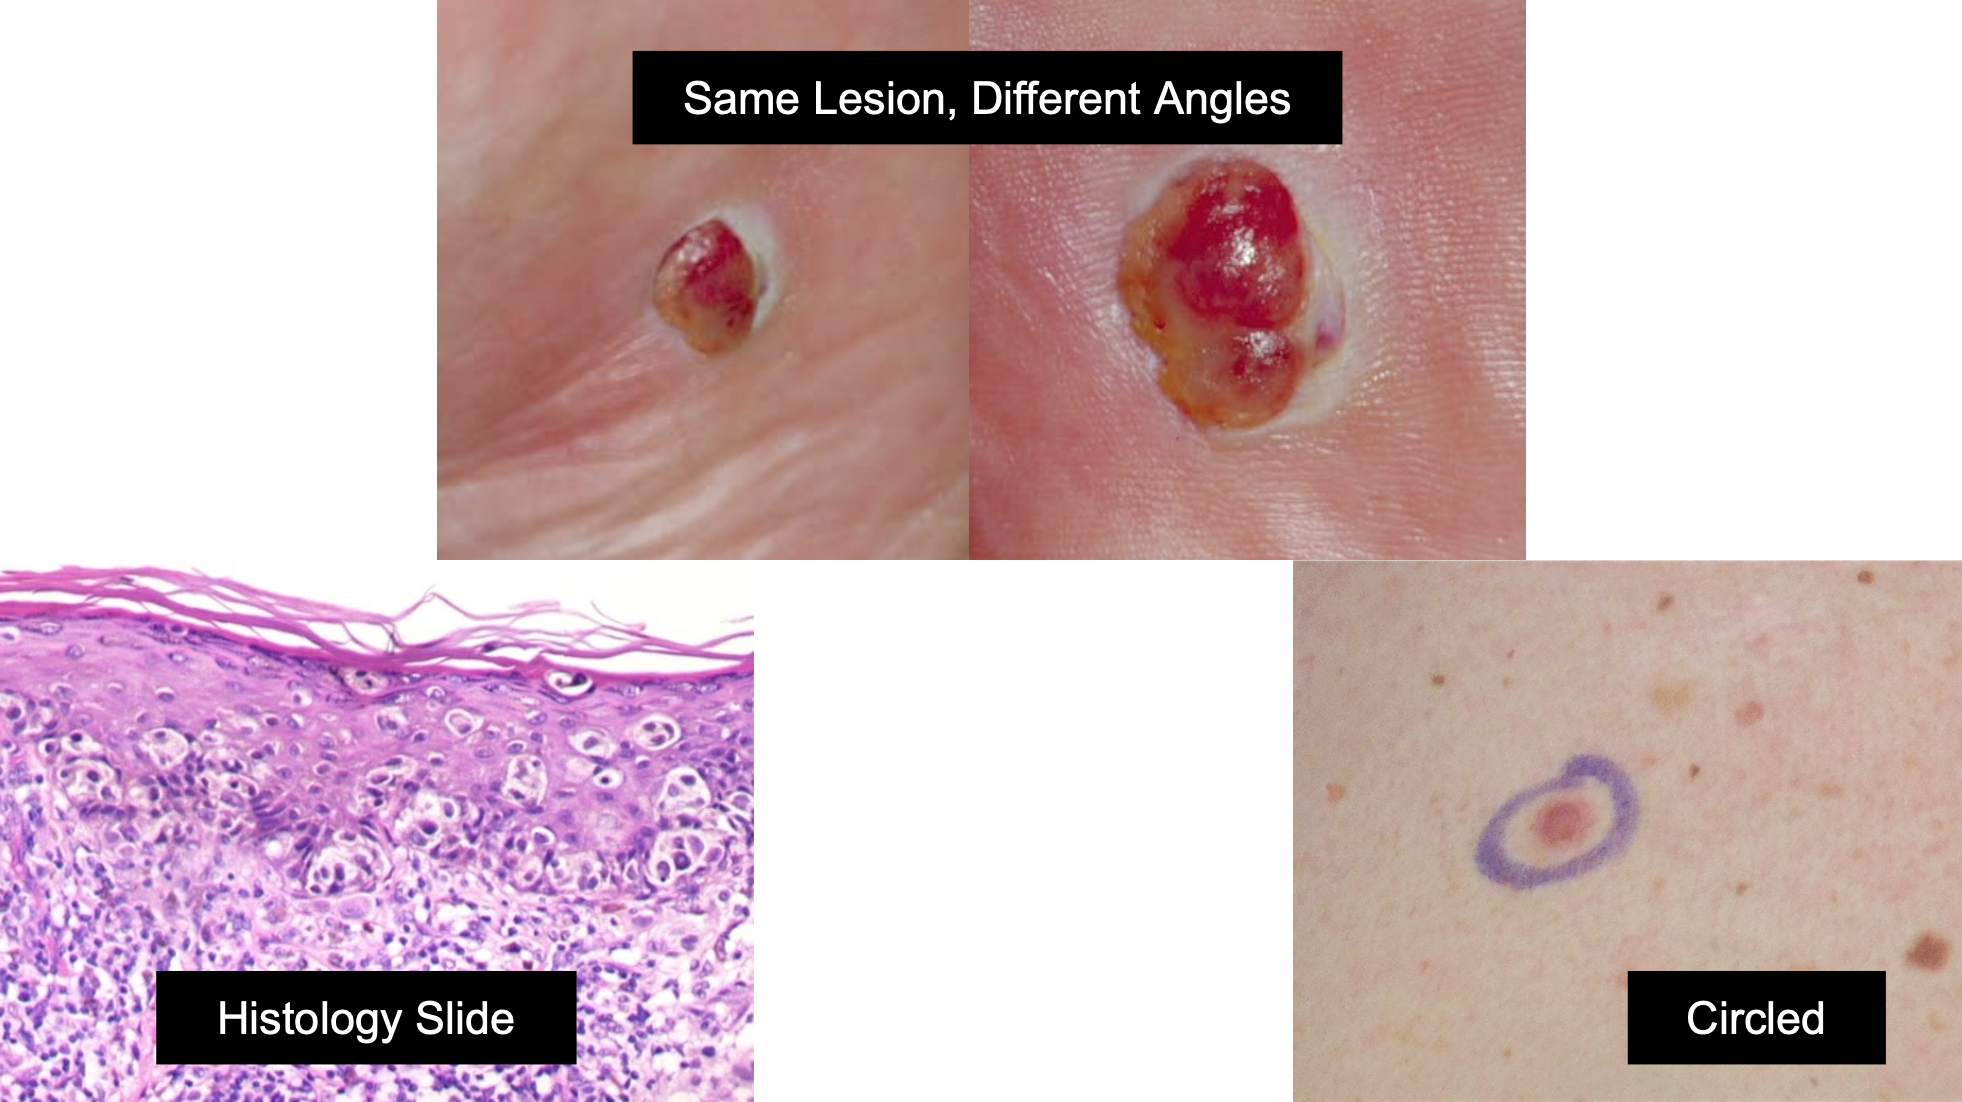
\includegraphics[width=\textwidth]{derm_data_problems}
\caption{Data Problems}
\vspace{12px}
Insert caption here
\label{fig:derm_data_problems}
\end{figure}

\begin{figure}

\includegraphics[width=\textwidth]{derm_nature}
\caption{Nature Publication}
\vspace{12px}
Insert caption here
\label{fig:derm_nature}
\end{figure}

\begin{figure}
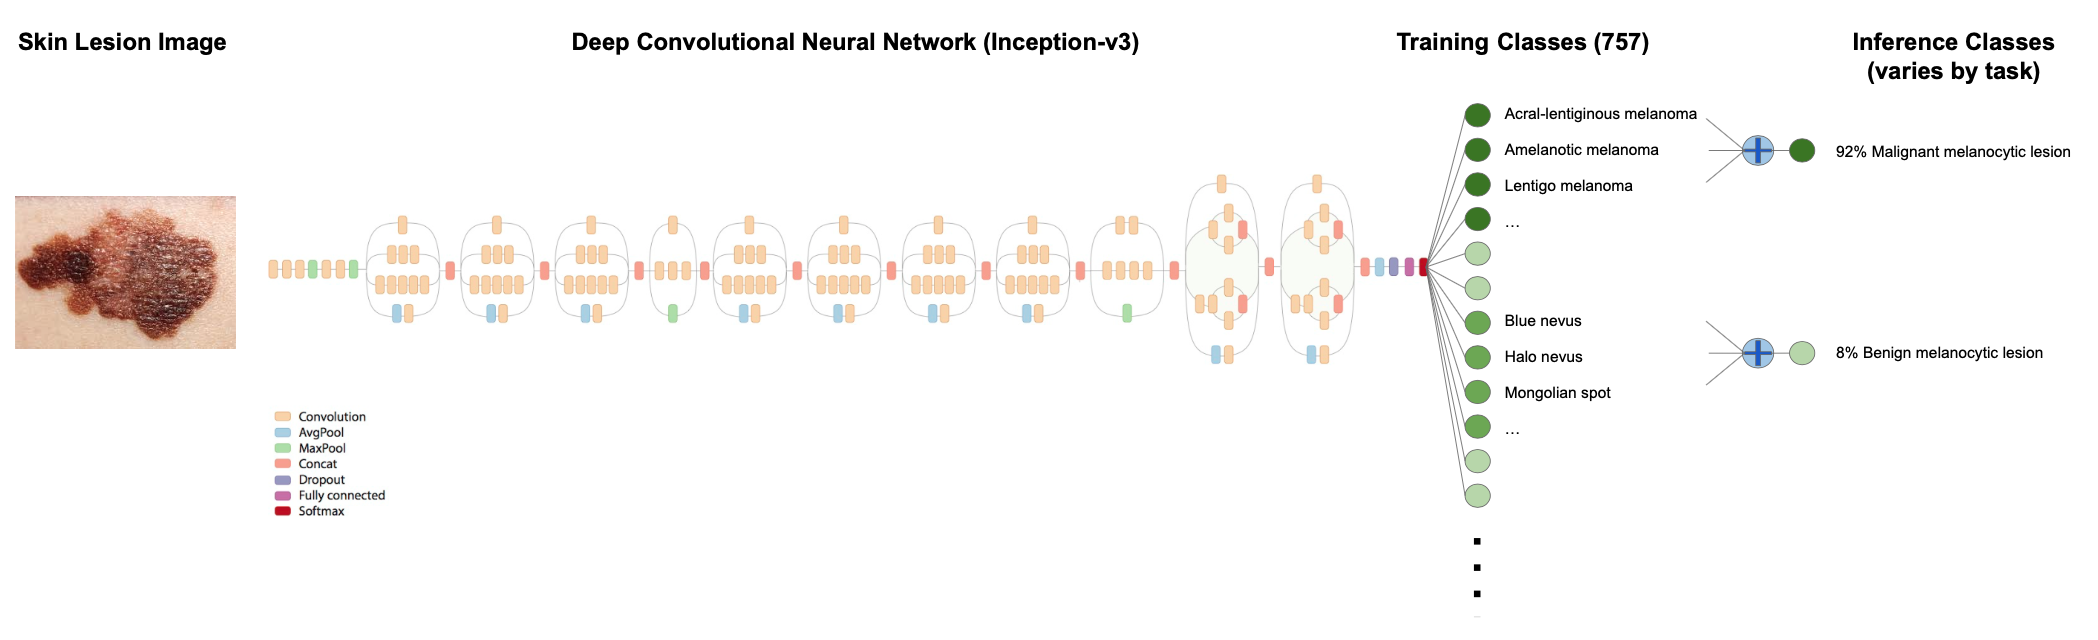
\includegraphics[width=\textwidth]{derm_cnn}
\caption{Model architecture}
\vspace{12px}
The classification method is a deep CNN. Data flow is from left to right: an image of a skin lesion (for example, melanoma) is sequentially warped into a probability distribution over clinical classes of skin disease using Google Inception v3 CNN architecture pretrained on the ImageNet dataset (1.28 million images over 1,000 generic object classes) and fine-tuned on a dataset of 129,450 skin lesions comprising 2,032 different diseases. The 757 training classes are defined using a novel taxonomy of skin disease and a partitioning algorithm that maps diseases into training classes (for example, acrolentiginous melanoma, amelanotic melanoma, lentigo melanoma). Inference classes are more general and are composed of one or more training classes (for example, malignant melanocytic lesions—the class of melanomas). The probability of an inference class is calculated by summing the probabilities of the training classes according to taxonomy structure (see Methods)
\label{fig:derm_cnn}
\end{figure}

\begin{figure}
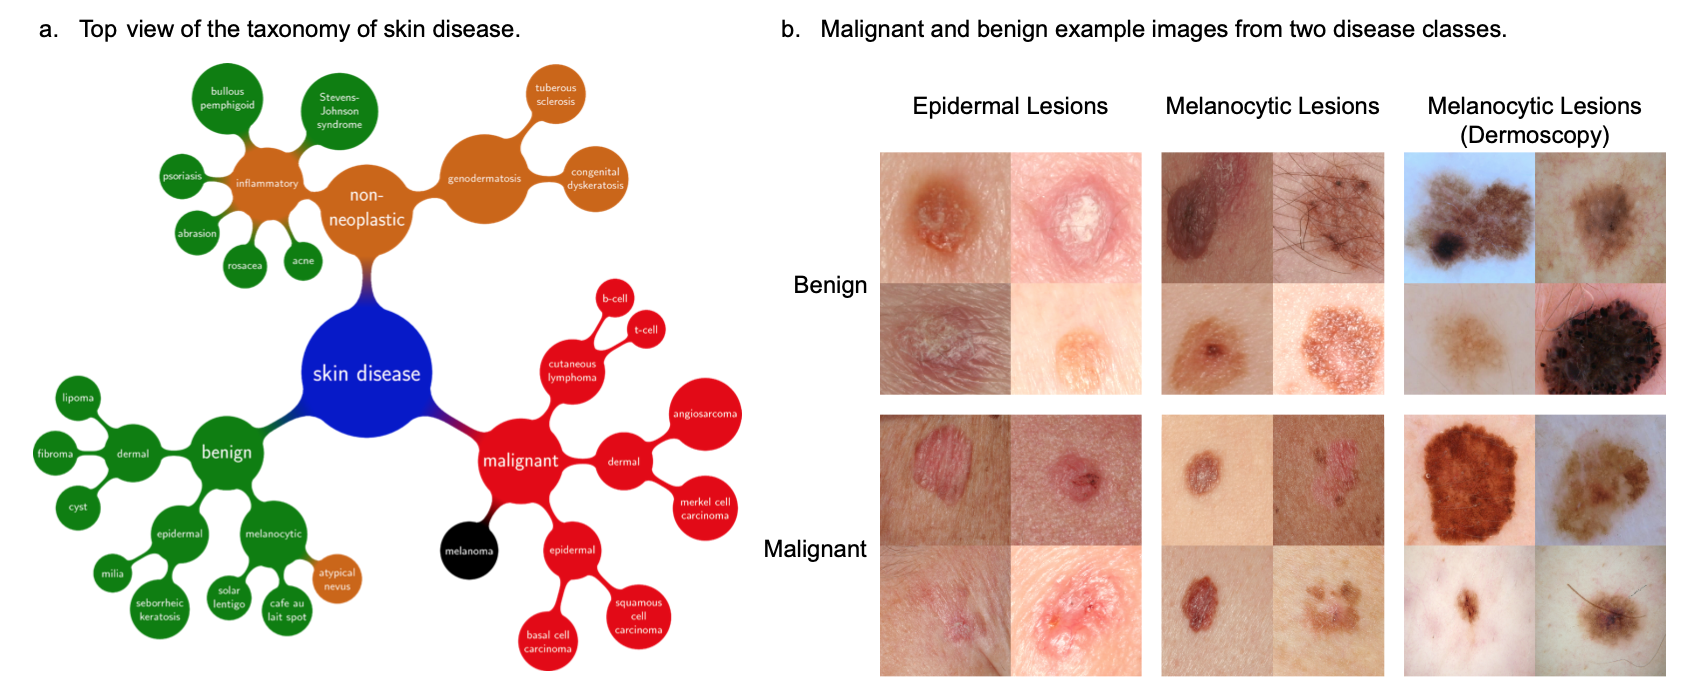
\includegraphics[width=\textwidth]{derm_taxonomy}
\caption{Taxonomy of skin diseases}
\vspace{12px}
(a) A subset of the top of the tree-structured taxonomy of skin disease. The full taxonomy contains 2,032 diseases and is organized based on visual and clinical similarity of diseases. Red indicates malignant, green indicates benign, and orange indicates conditions that can be either. Black indicates melanoma. The first two levels of the taxonomy are used in validation. Testing is restricted to the tasks shown in (b). (b) Malignant and benign example images from two disease classes. These test images highlight the difficulty of malignant versus benign discernment for the three medically critical classification tasks considered: epidermal lesions, melanocytic lesions and melanocytic lesions visualized with a dermoscope. Example images reprinted with permission from the Edinburgh Dermofit Library.
\label{fig:derm_taxonomy}
\end{figure}

\begin{figure}
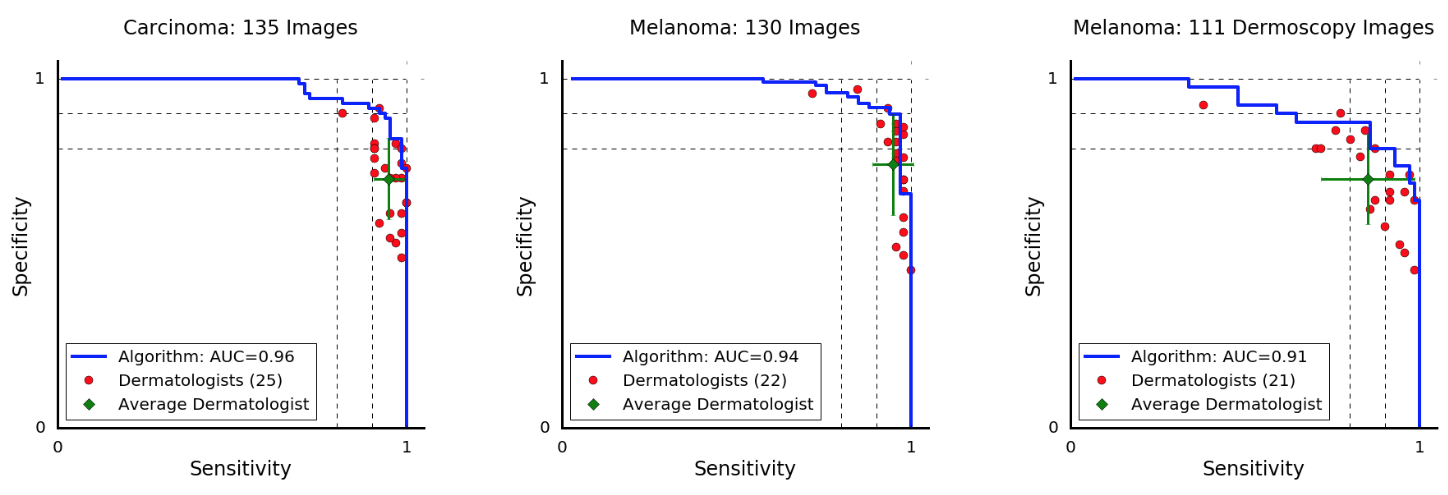
\includegraphics[width=\textwidth]{derm_sens_spec}
\caption{Sensitivity and specificity comparison}
\vspace{12px}
The deep learning CNN outperforms the average of the dermatologists at skin cancer classification using photographic and dermoscopic images. The CNN is tested against at least 21 dermatologists at keratinocyte carcinoma and melanoma recognition. For each test, previously unseen, biopsy-proven images of lesions are displayed, and dermatologists are asked if they would: biopsy/treat the lesion or reassure the patient. Sensitivity, the true positive rate, and specificity, the true negative rate, measure performance. A dermatologist outputs a single prediction per image and is thus represented by a single red point. The green points are the average of the dermatologists for each task, with error bars denoting one standard deviation (calculated from $n$ = 25, 22 and 21 tested dermatologists for keratinocyte carcinoma, melanoma and melanoma under dermoscopy, respectively). The CNN outputs a malignancy probability $p$ per image. The prediction $\hat{y}$ for any image given the threshold probability $t$ is $\hat{y} = p \geq t$, and the blue curve is drawn by sweeping $t$ in the interval $[0, 1]$. The CNN achieves superior performance to a dermatologist if the sensitivity–specificity point of the dermatologist lies below the blue curve, which most do. Epidermal test: 65 keratinocyte carcinomas and 70 benign seborrheic keratoses. Melanocytic test: 33 malignant melanomas and 97 benign nevi. A second melanocytic test using dermoscopic images is displayed for comparison: 71 malignant and 40 benign. The slight performance decrease reflects differences in the difficulty of the images tested rather than the diagnostic accuracies of visual versus dermoscopic examination.
\label{fig:derm_sens_spec}
\end{figure}

\begin{figure}
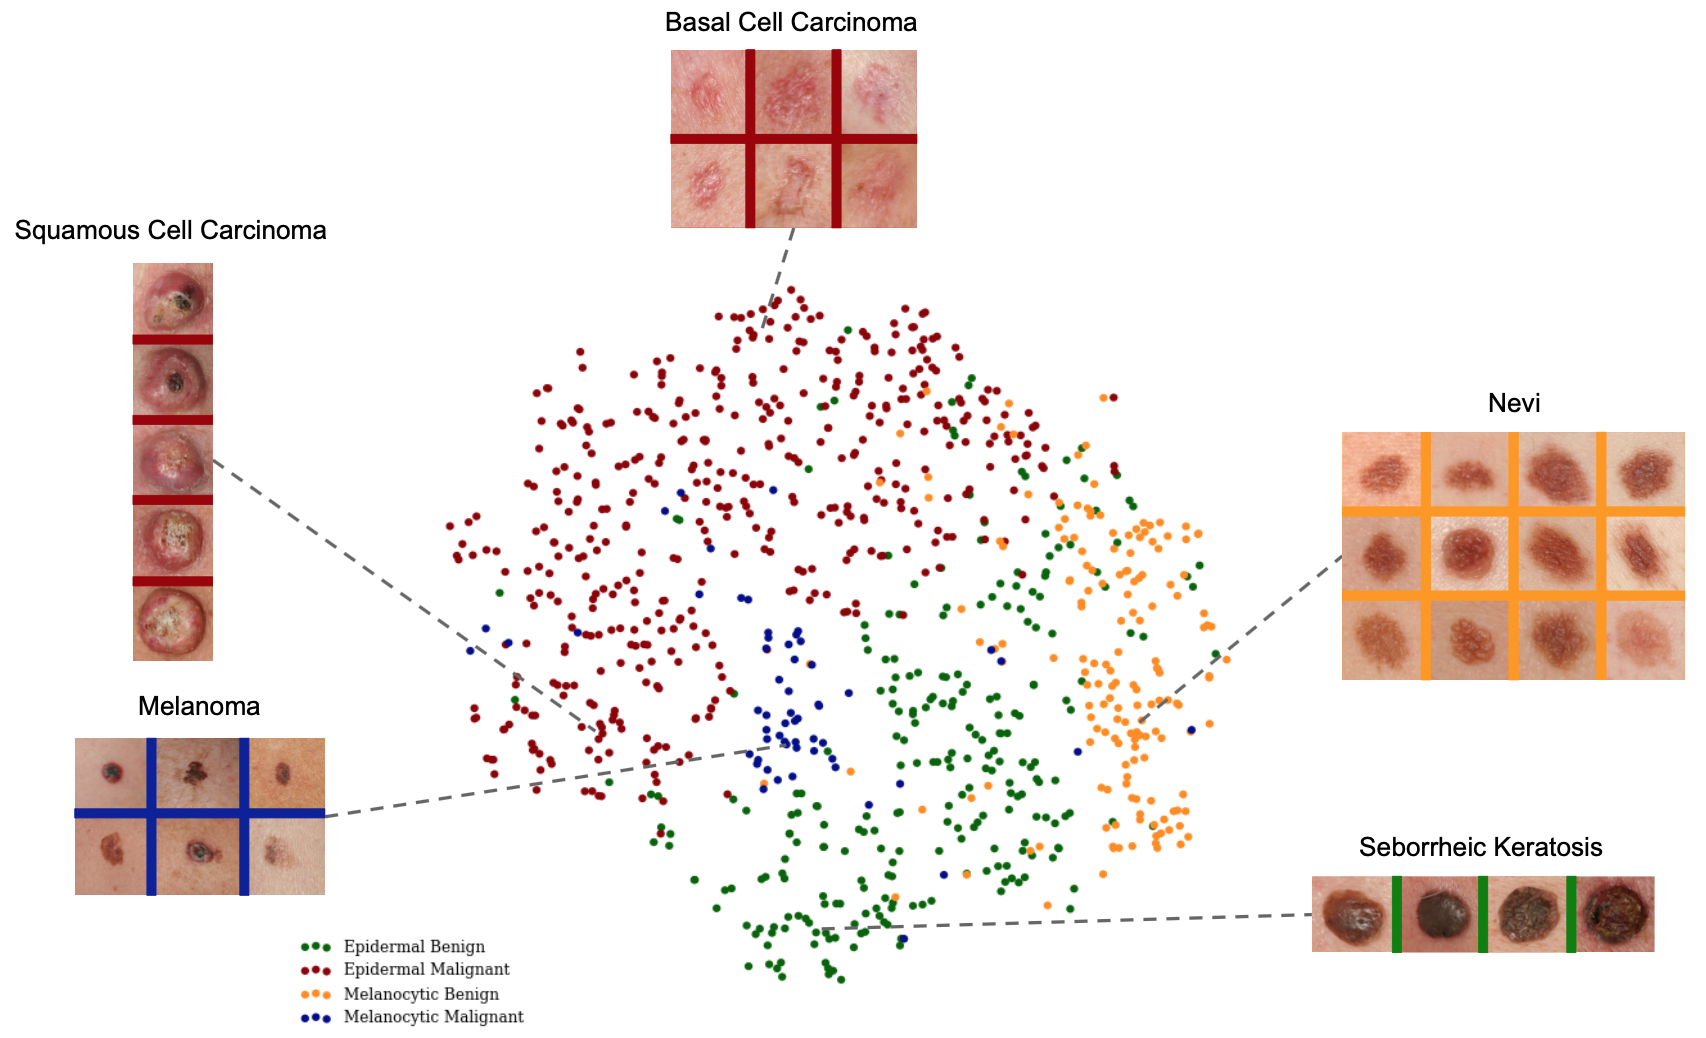
\includegraphics[width=\textwidth]{derm_tsne}
\caption{Low dimensional embedding of learned features}
\vspace{12px}
Here the CNN’s internal representation for four important disease classes is shown by applying t-SNE, a method for visualizing high-dimensional data, to the last hidden layer representation in the CNN of the biopsy-proven photographic test sets (932 images). Colored point clouds represent the different disease categories, showing how the algorithm clusters the diseases. Insets show images corresponding to various points. Images reprinted with permission from the Edinburgh Dermofit Library.
\label{fig:derm_tsne}
\end{figure}

\begin{figure}
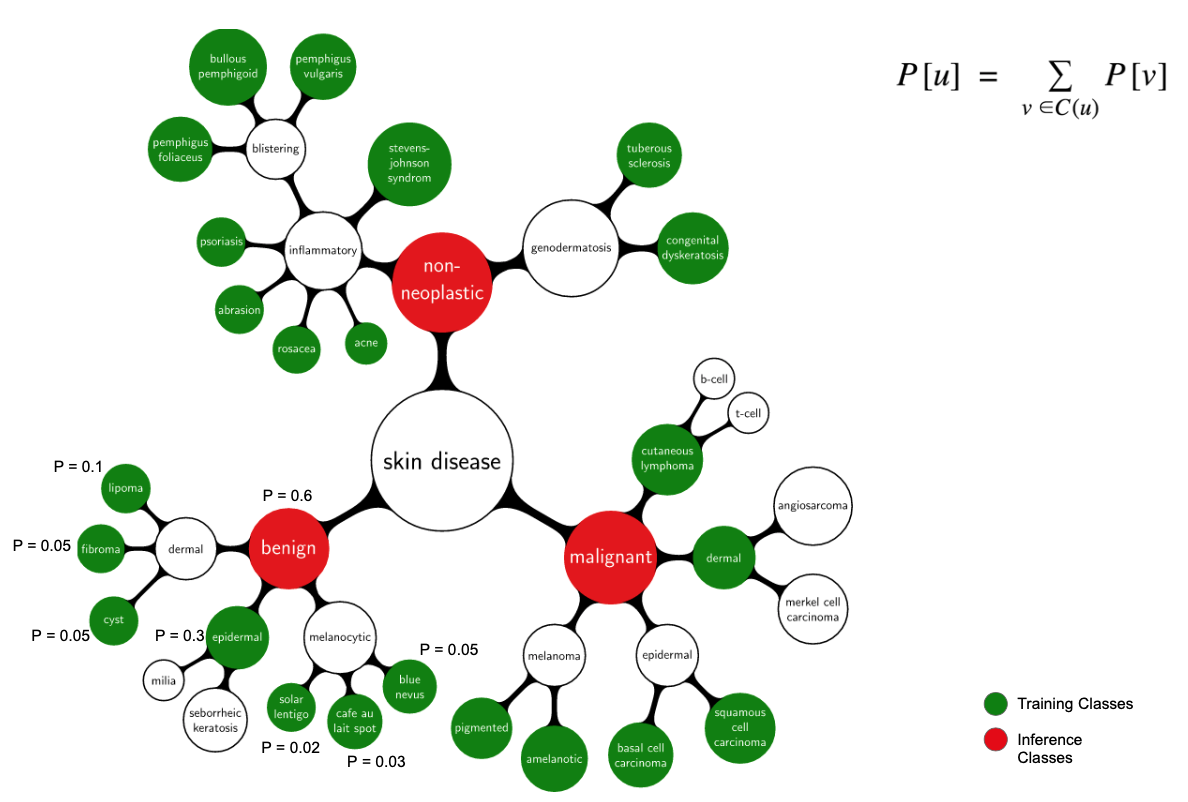
\includegraphics[width=\textwidth]{derm_tree_inference}
\caption{Tree inference}
\vspace{12px}
Illustrative example of the inference procedure using a subset of the taxonomy and mock training/inference classes. Inference classes (for example, malignant and benign lesions) correspond to the red nodes in the tree. Training classes (for example, amelanotic melanoma, blue nevus), which were determined using the partitioning algorithm with $maxClassSize = 1000$, correspond to the green nodes in the tree. White nodes represent either nodes that are contained in an ancestor node’s training class or nodes that are too large to be individual training classes. The equation represents the relationship between the probability of a parent node, $u$, and its children, $C(u)$; the sum of the child probabilities equals the probability of the parent. The CNN outputs a distribution over the training nodes. To recover the probability of any inference node it therefore suffices to sum the probabilities of the training nodes that are its descendants. A numerical example is shown for the benign inference class: $P_{benign} = 0.6 = 0.1 + 0.05 + 0.05 + 0.3 + 0.02 + 0.03 + 0.05$.
\label{fig:derm_tree_inference}
\end{figure}

\begin{figure}
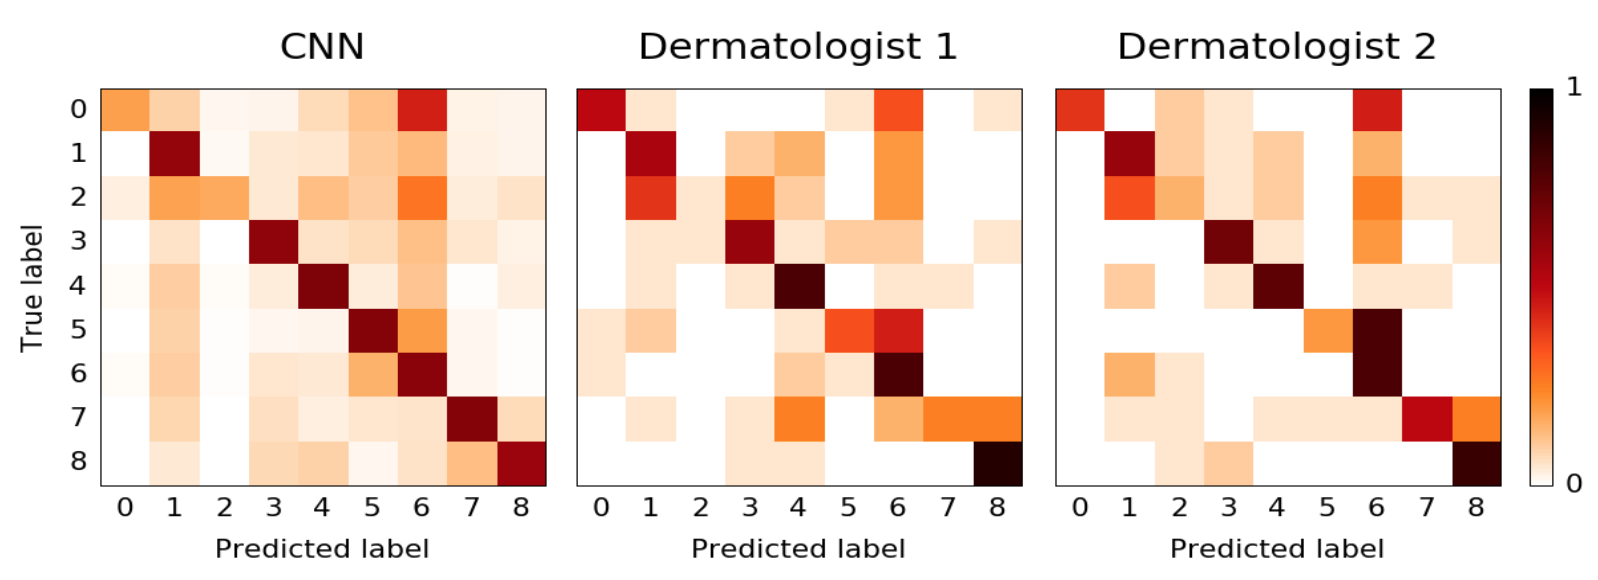
\includegraphics[width=\textwidth]{derm_confusion_matrix}
\caption{Confusion matrix comparison}
\vspace{12px}
Confusion matrices for the CNN and both dermatologists for the nine-way classification task of the second validation strategy reveal similarities in misclassification between human experts and the CNN. Element (i, j) of each confusion matrix represents the empirical probability of predicting class j given that the ground truth was class i, with i and j referencing classes from Extended Data Table 2d. Note that both the CNN and the dermatologists noticeably confuse benign and malignant melanocytic lesions—classes 7 and 8—with each other, with dermatologists erring on the side of predicting malignant. The distribution across column 6—inflammatory conditions—is pronounced in all three plots, demonstrating that many lesions are easily confused with this class. The distribution across row 2 in all three plots shows the difficulty of classifying malignant dermal tumours, which appear as little more than cutaneous nodules under the skin. The dermatologist matrices are each computed using the 180 images from the nine-way validation set. The CNN matrix is computed using a random sample of 684 images (equally distributed across the nine classes) from the validation set.
\label{fig:derm_confusion_matrix}
\end{figure}

\begin{figure}
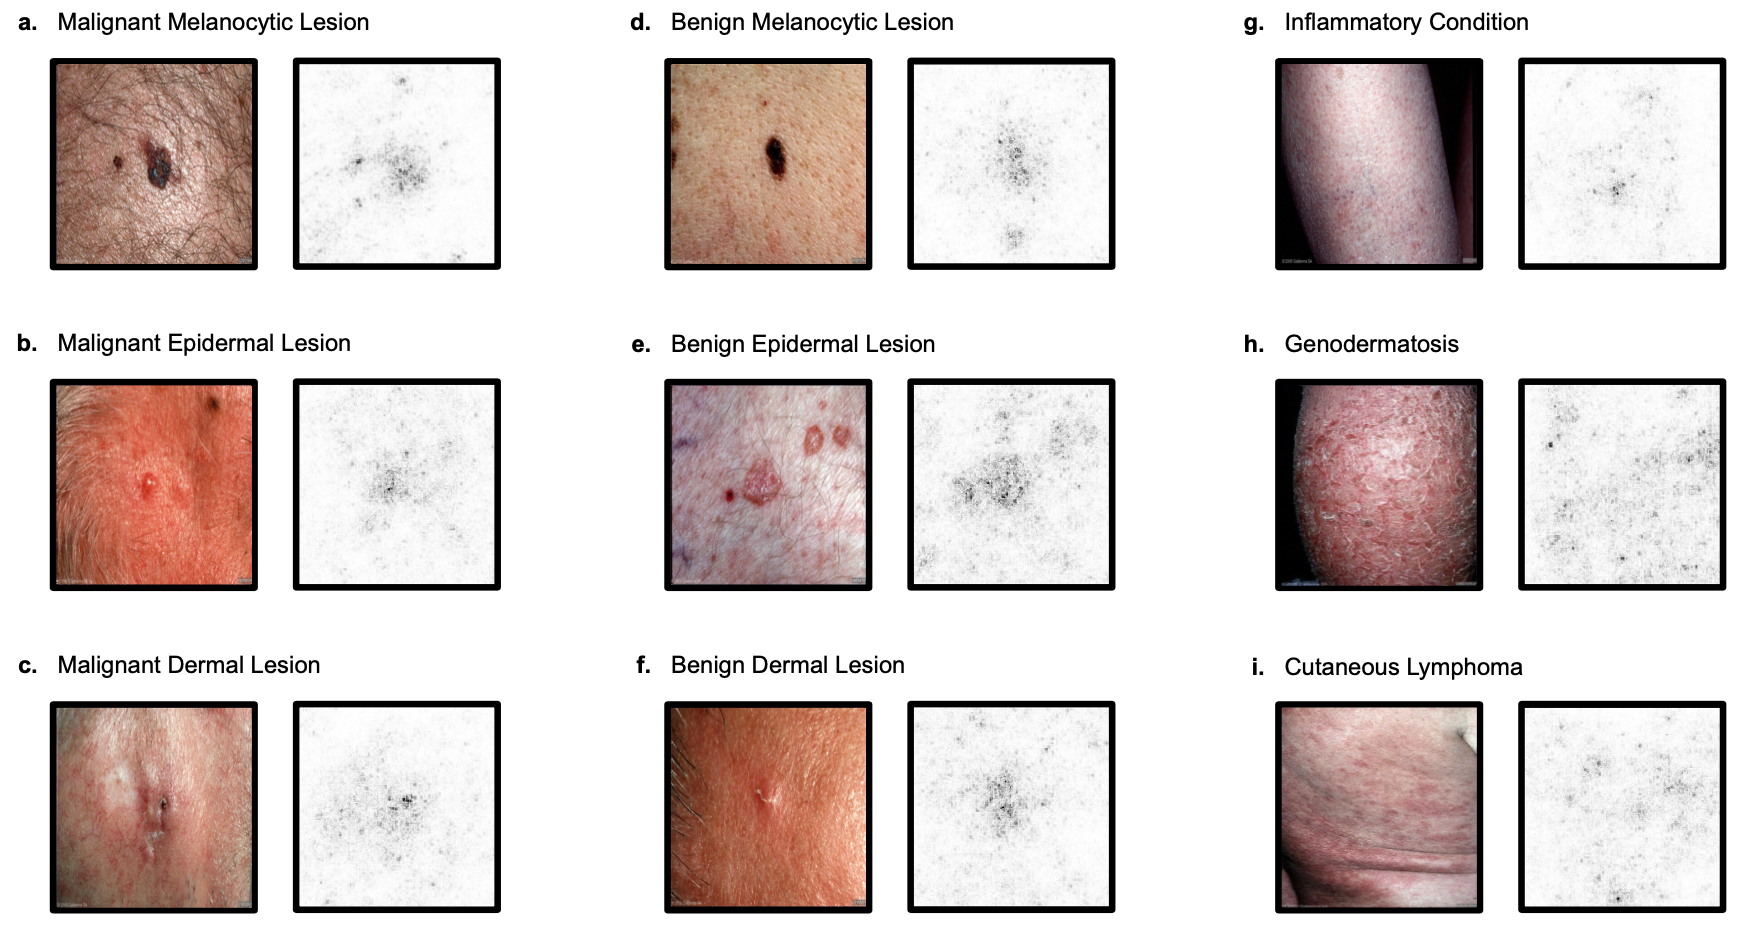
\includegraphics[width=\textwidth]{derm_saliency}
\caption{Saliency maps for nine example lesions}
\vspace{12px}
Saliency maps for example images from each of the nine clinical disease classes of the second validation strategy reveal the pixels that most influence a CNN’s prediction. Saliency maps show the pixel gradients with respect to the CNN’s loss function. Darker pixels represent those with more influence. Conditions with a single lesion (a–f) tend to exhibit tight saliency maps centred around the lesion. Conditions with spreading lesions (g–i) exhibit saliency maps that similarly occupy multiple points of interest in the images. (a) Malignant melanocytic lesion. (b) Malignant epidermal lesion. (c) Malignant dermal lesion. (d) Benign melanocytic lesion. (e) Benign epidermal lesion. (f) Benign dermal lesion. (g) Inflammatory condition. (h) Genodermatosis. (i) Cutaneous lymphoma.
\label{fig:derm_saliency}
\end{figure}

To take advantage of fine-grained information contained in the structure of the taxonomy, an algorithm was made (Extended Data Algorithm 1) to partition the diseases into fine-grained training classes (e.g. amelanotic melanoma and acrolentiginous melanoma). During inference, the CNN outputs a probability distribution over these fine classes. To recover the probabilities for coarser-level classes of interest (e.g. melanoma), the probabilities of their descendants are added. See Figure \ref{fig:derm_tree_inference} for more details.

The algorithm’s effectiveness is validated in two ways, using nine-fold cross validation. First, it is validated with a three-class disease partition - the level-1 nodes of the taxonomy - representing benign lesions, malignant lesions, and non-neoplastic lesions. Here the CNN achieves 72.1 ± 0.9\% overall accuracy (the average of individual inference class accuracies) and two dermatologists attain 65.56\% and 66.0\% accuracy on a subset of the validation set. Second, it is validated with a nine-class disease partition - the level-2 nodes - such that the diseases of each class have similar medical treatment plans. The CNN achieves 55.4 ± 1.7\% overall accuracy whereas the same two dermatologists attain 53.3\% and 55.0\% accuracy. A CNN trained on a finer disease partition performs better than one trained directly on three or nine classes (see Extended Data Table 1), demonstrating the effectiveness of the partitioning algorithm. Since validation set images are labeled by dermatologists but not necessarily biopsy-proven, this metric is inconclusive, and instead serves to show that the CNN is learning relevant information.

For conclusiveness, the model and dermatologists are tested using strictly biopsy-proven images on medically significant use cases: distinguishing malignant versus benign (1) epidermal lesions (malignant carcinoma vs benign seborrheic keratosis) and (2) melanocytic lesions (malignant melanoma vs benign nevi). For (2), one test is comprised of standard images and the other dermoscopy images, which reflect two steps that a dermatologist might pursue to obtain a clinical impression. The same CNN is used across all three tasks. Figure \ref{fig:derm_taxonomy}(b) shows a few example images from each case, demonstrating the difficulty in distinguishing between malignant and benign lesions, which share many visual features. The comparison metrics used are sensitivity and specificity (SS):

$$sensitivity = \frac{TP}{P}$$
$$specificity = \frac{TN}{N}$$

Where $TP$ (true positives) is the number of correctly predicted malignant lesions, $P$ is the number of malignant lesions shown, $TN$ (true negatives) is the number of correctly predicted benign lesions, and $N$ is the number of benign lesions shown. When a test set is fed through the CNN, it outputs a probability, $p$, of malignancy, per image. The sensitivity and specificity given these probabilities are computed by choosing a threshold probability $t$ such that the prediction $y$ for each image is given by $y = p > t$. Varying $t$ in the interval $[0,1]$ generates a curve of sensitivities and specificities that the CNN can achieve.

Figure \ref{fig:derm_sens_spec}(a) shows a direct performance comparison between the CNN and over 81 board-certified dermatologists on epidermal and melanocytic lesion classification. For each image the dermatologists are asked whether to (a) biopsy/treat the lesion or (b) reassure the patient. Each red point on the plots represents the SS of a single dermatologist. The CNN outperforms any dermatologist whose SS point falls below the CNN’s blue curve - most do. The green points represents the average dermatologist (average SS of all red points), with error bars denoting one standard deviation. The area-under-the-curve (AUC) for each case is over 91\%. The data for this comparison (135 epidermal, 130 melanocytic, and 111 melanocytic-dermoscopy images) are sampled from the full test sets. Plotted in Figure \ref{fig:derm_sens_spec}(a) are the SS curves for the entire test set of biopsy-labeled images comprised of 707 epidermal, 225 melanocytic, and 1,010 melanocytic-dermoscopy images. From Figure \ref{fig:derm_sens_spec}(a) to Figure \ref{fig:derm_sens_spec}(b) there are negligible changes in AUC (<0.03), validating the reliability of the results on a larger dataset. In a separate analysis with similar results (see Methods) dermatologists are asked if they believe a lesion is (a) malignant or (b) benign.

Using t-SNE \cite{van2008visualizing}, a technique for visualizing high-dimensional data, in Figure \ref{fig:derm_tsne} the features learned by the CNN that allow it to classify skin lesions accurately are shown. Each point represents a skin lesion image (either epidermal or melanocytic) projected from the 2048-dimensional output of the CNN’s last hidden layer into two dimensions.  There are clusters of points of the same clinical classes - insets show thumbnail images of different diseases. Basal and squamous cell carcinomas are split across the malignant epidermal point cloud. Melanomas lie in the center, in contrast to nevi which lie on the right. Similarly, seborrheic keratoses lie across from their malignant counterparts. 

Here the effectiveness of deep learning in dermatology is demonstrated - a technique which is applied to both general skin conditions and specific cancers. Using a single deep convolutional neural network trained at general skin lesion classification, the performance of over 21 tested dermatologists across three critical diagnostic tasks is matched: carcinoma classification, melanoma classification, and melanoma classification under dermoscopy. This fast, scalable method can be deployed on mobile devices, broadening the scope of primary care practice, and augmenting clinical decision-making for dermatology specialists. Further research is necessary to evaluate performance in a clinical setting, as a dermatologist’s clinical impression involves more than visual inspection of an isolated lesion. However, the ability to classify skin lesion images with the accuracy of a board-certified dermatologist has the potential to dramatically expand access to vital medical care. This method is primarily constrained by data and can classify many visual conditions if sufficient training examples exist. Deep learning is agnostic to the type of image data used and could be adapted to other specialties, including ophthalmology, otolaryngology, radiology, and pathology. 

\subsection{Datasets}
The dataset comes from a combination of open-access dermatology repositories, the ISIC Dermoscopic Archive, the Edinburgh Dermofit Library, and data from the Stanford Hospital. The images from the online open-access dermatology repositories are annotated by dermatologists, not necessarily through biopsy. The ISIC Archive data used is composed strictly of melanocytic lesions that are biopsy-proven and annotated as malignant or benign. The Edinburgh Dermofit Library and data from the Stanford Hospital are biopsy-proven and annotated by individual disease names (e.g. actinic keratosis). 

\subsection{Taxonomy}
The taxonomy represents 2,032 individual diseases arranged in a tree structure with its three root nodes representing general disease classes: (1) benign lesions, (2) malignant lesions, and (3) non-neoplastic lesions (Figure \ref{fig:derm_taxonomy}(b)). It was derived by dermatologists using a bottom-up procedure: individual diseases, initialized as leaf nodes, were merged based on clinical and visual similarity, until the entire structure was connected. This aspect of the taxonomy makes it useful in generating training classes that are both well-suited for machine learning classifiers and medically relevant. The root nodes are used in the first validation strategy and represent the most general partition. The children of the root nodes (i.e. malignant melanocytic lesions) are used in the second validation strategy, and represent disease classes that have similar clinical treatment plans.

\subsection{Data Preparation}
Blurry images and far-away images were removed from the test and validation sets, but still used in training. The dataset contains sets of images corresponding to the same lesion but from multiple viewpoints, or multiple images of similar lesions on the same person. While this is useful training data, extensive care was taken to ensure that these sets were not split between the training and validation sets. Using image EXIF metadata, repository specific information, and nearest neighbor image retrieval with CNN features, an undirected graph connecting any pair of images that were determined to be similar was created. Connected components of this graph were not allowed to straddle the train/validation split and were randomly assigned to either train or validation. The test sets all came from independent, high-quality repositories of biopsy-proven images - the Stanford Hospital, the University of Edinburgh Dermofit Image Library, and the ISIC Dermoscopic Archive. No overlap (i.e. same lesion multiple viewpoints) exists between the test sets and the training/validation data.

\subsection{Sample Selection}
The epidermal, melanocytic, and melanocytic-dermoscopic tests of Figure \ref{fig:derm_sens_spec}(a) used 135 (65 malignant, 70 benign), 130 (33 malignant, 97 benign), and 111 (71 malignant, 40 benign) images, respectively. Their counterparts of Figure \ref{fig:derm_sens_spec}(b) used 707 (450 malignant, 257 benign), 225 (58 malignant, 167 benign), and 1010 (88 malignant, 922 benign) images, respectively. The number of images used for Figure \ref{fig:derm_sens_spec}(b) was based on the availability of biopsy-labeled data (i.e. malignant melanocytic lesions are exceedingly rare compared to benign melanocytic lesions). These numbers are statistically justified by the standards of the ILSVRC computer vision challenge6, which has 50-100 images per class for validation and test sets. For (a), 140 images were randomly selected from each set of (b), and a non-tested dermatologist removed any images of insufficient resolution (while the network accepts 299 x 299 image inputs, humans require larger images for clarity).

\subsection{Disease Partitioning Algorithm}
The algorithm that partitions the individual diseases into training classes is outlined more formally in Extended Data Algorithm 1. It is a recursive algorithm, designed to leverage the taxonomy to generate training classes whose individual diseases are clinically and visually similar. The algorithm forces the average generated training class size to be slightly less than its only hyperparameter, $maxClassSize$. Together these components strike a balance between (1) generating training classes that are overly-fine grained and don’t have sufficient data to be learned properly, (2) generating training classes that are too coarse, too data abundant, and bias the algorithm towards them. With $maxClassSize = 1000$ this algorithm yields a disease partition of 757 classes. All training classes are descendants of inference classes.

\subsection{Training Algorithm}
Google’s Inception-v3 CNN architecture pre-trained to 93.33\% top-5 accuracy on the 1000 object classes (1.28M images) of the 2014 ImageNet Challenge following \cite{szegedy2016rethinking} was used. The final classification layer is removed from the network and the net is retrained with the dataset, fine-tuning the parameters across all layers. During training each image is resized to 299 x 299 pixels in order to make it compatible with the original dimensions of the Inception-v3 network architecture and leverage the natural-image features learned by the ImageNet pretrained network. This procedure, known as transfer learning, is optimal given the amount of data available.

The CNN is trained using backpropagation. All layers of the network are fine-tuned using the same global learning rate of 0.001 and a decay factor of 16 every 30 epochs. RMSProp is used with decay of 0.9, momentum of 0.9, and epsilon of 0.1. Google’s TensorFlow \cite{abadi2016tensorflow} deep learning framework is used to train, validate, and test the network. During training, images are augmented by a factor of 720. Each image is rotated randomly between 0 and 359 degrees. The largest upright inscribed rectangle is then cropped from the image, and is flipped vertically with a probability of 1/2. 

\subsection{Inference Algorithm}
Each training class is represented by a node in the taxonomy, and subsequently, all descendants. Each inference class is a node which has as its descendants some set of training nodes. An illustrative example is shown in Figure \ref{fig:derm_tree_inference}, with red nodes as inference classes and green nodes as training classes. Given an input image, the CNN outputs a probability distribution over the training nodes. Probabilities over the taxonomy follow:

$$P(u) = \sum_{v \in C(u)}{P(v)}$$

Where $u$ is any node, $P(u)$ is the probability of $u$, and $C(u)$ are the child nodes of $u$. Thus to recover the probability of any inference node, the probabilities of its descendant training nodes are added. Note that in the validation strategies all training classes are summed into inference classes. However in the binary classification cases, the images in question are known to be either melanocytic or epidermal and so only the training classes which are descendants of either melanocytic or epidermal are used.

\subsection{Confusion Matrices}
Figure \ref{fig:derm_confusion_matrix} shows the confusion matrix of the model over the nine classes of the second validation strategy (Extended Data Table 1(d)) in comparison to the two tested dermatologists. This demonstrates the misclassification similarity between the CNN and human experts. Element $(i, j)$ of each confusion matrix represents the empirical probability of predicting class $j$ given that the ground truth was class i. Classes 7 and 8 - benign and malignant melanocytic lesions - are often confused for each other. Many images are mistaken as class 6, the inflammatory class, due to the high variability of diseases in this category. Note how easily malignant dermal tumors are confused for other classes, by both the CNN and dermatologists. They are essentially nodules under the skin that are challenging to visually diagnose. 

\subsection{Saliency Maps}
To visualize the pixels that a network is fixating on for its prediction, saliency maps are generated, shown in Figure \ref{fig:derm_saliency}, for example images of the nine classes of Extended Data Table 1(d). Backpropagation is an application of the chain rule of calculus to compute loss gradients for all weights in the network. The loss gradient can also be backpropagated to the input data layer. By taking the $L_1$ norm of this input layer loss gradient across the RGB channels, the resulting heat map intuitively represents the importance of each pixel for diagnosis. As can be seen, the network fixates most of its attention on the lesions themselves and ignores background and healthy skin.

\subsection{Sensitivity-Specificity Curves with different question}
The CNN's sensitivity and specificity were compared to that of over 21 dermatologists on the three diagnostic tasks of Figure \ref{fig:derm_sens_spec}. In that analysis each dermatologist was asked if they would (a) biopsy/treat the lesion, or (b) reassure the patient. This choice of question reflects the actual in-clinic task that dermatologists must perform - deciding whether or not to continue medically analyzing a lesion. A similar question to ask a dermatologist, though less clinically relevant, is if they believe a lesion is (a) malignant, or (b) benign. The results of this analysis are shown in Extended Data Figure 4. As in the main Figure \ref{fig:derm_sens_spec}, the CNN is on par with the performance of the dermatologists and outperforms the average. In the epidermal lesions test the CNN is just above one standard deviation above the average dermatologist, and in both melanocytic lesion tests the CNN is just below one standard deviation above the average dermatologist. 

\subsection{Use of human subjects}
All human subjects were board-certified dermatologists that consented to take the tests. This study was approved by the Stanford Institutional Review Board, under trial registration number 36050.